\documentclass{ctexart}

% 导言区
\usepackage[colorlinks,linkcolor=blue,bookmarksopen=true,bookmarksnumbered=true,citecolor=blue]{hyperref}             % 目录点击跳转
\usepackage[]{amsmath}
\usepackage{cite}
\usepackage[colorlinks,linkcolor=blue]{hyperref}
\usepackage{siunitx}
\usepackage{graphicx}
\usepackage{subfigure}
\usepackage{float}


\newcommand\subtitle[1]{\rightline{\small #1}} 


\setlength{\parindent}{4em}
\title{不幸掉进黑洞会发生什么?\\ \subtitle{——普通天文学课程期末报告}  } % 添加标题
\author{郑卜凡\quad2021302022016}                     % 添加作者
\date{\today}                             %最后更新日期


\begin{document}
    \maketitle              %制作封面
    \begin{abstract}
        简略的论述了黑洞的一些相关知识以及科幻片中对于黑洞的想象。基于相关的一些论文以及书籍作品讨论了如果人不幸掉入黑洞他/她会经历什么?黑洞外的人观察到了
        什么?
    \end{abstract}
    \tableofcontents        %制作目录
    \section{什么是黑洞?}
    \subsection{黑洞的历史由来}
        其实\textbf{黑洞}这个概念历史上并不新鲜。早在1784年,John Michell\footnote{除了一些熟知的译名,为了消除歧义,本文中涉及到的英文名全部用原始英文代替。}根据牛顿的微粒说,认为光由粒子构成,那么自然的想到这些粒子便会在靠近星体时由于万有
        引力定律被吸引。米歇尔设想了一个极限情形,当恒星的质量大到一定程度时,“所有的光都会被恒星的引力拖拽回去”。这意味着这颗恒星所辐射出的光永远无法逃逸,这颗恒星永远无法被看见,
        Michell称之为“暗星(dark star)”。1976年,法国大革命期间,法国数学家Laplace也独立的得出了与Michell类似的结论,并在他著作《宇宙体系论》({\itshape Exposition du syst\'eme du monde})中记录了这一发现。\cite{montgomery2009michell}
        不过后来Laplace并没有坚持他的这一想法, 可能是后来光的波动学说打败了光的微粒学说, 也或者是他仅仅对此失去了兴趣, 总之后来他在《宇宙体系论》的第二版中删除了这一论述。

        相反Michell在1784年发表的那篇论文中提到了虽然“暗星”无法被直接看见,但是其周围的星体却会因为它强大的吸引力而随之运动,从而可以用来证明它的存在性。\cite{1784michell}
        而这也是当今天文学家追踪黑洞的有效手段之一!

        尽管Michell和Laplace在当时都走在了时代的前沿,但是由于时代的限制,他们的论断是基于万有引力定律以及错误的光理论得出的,而且当时大众还不完全接受万有引力
        定律的正确性,仍然迷信的认为行星收到的引力是来自于看不见的“天使”的推动。\cite{feynman2011feynman}而且它们都只考虑了密度和太阳相同但体积比太阳大很多的恒星可能会变成暗星(Michell的计算认为直径是太阳的500倍),
        却没有考虑体积非常小,但是密度很大的星体变成所谓“暗星”的可能性,在当今宇宙中,超大恒星的密度要远远小于他们的想象。这或者也是因为时代的限制,当时的天文学家认为所有的星体的密度
        与地球和太阳都差不多。
        
    \subsection{人类对黑洞的探索历程}

    读者或多或少都见过下面的推导,考虑一个质量为$M$半径为$R$的星体,根据万有引力定律可以计算出其最小逃逸速度也即第二宇宙速度为:
    \begin{equation}
        v_2=\sqrt{\frac{2GM}{R}}
    \end{equation}
    
    我们假若把上面的$v_1$替换成光速,字面意义上看就是在这一情况下光都无法逃脱,我们可以得到:
    \begin{equation}
        R_s=\frac{2GM}{c^2}
    \end{equation}
    
    巧合的是,这一简单的、依赖于万有引力定律的粗略计算竟然正是依赖于广义相对论给出的\textbf{施瓦西半径(Schwarzschild Radius)}的精确形式!在这一半径内的物理
    恰恰是和Michell所想的那样连光都无法逃脱。难以置信,两百多年前,Michell和Laplace根据这一 简单的计算给出了黑洞的雏形——“暗星”,又过了一百多年,广义相对论的出现让关于“暗星”的讨论重新走在了历史前沿。
    
    Schwarzschild最初的目标是去为求解广义相对论方程发展一套通用的数学方法,他最先考虑了最简单的情形求出了点质量分布和各向同性球分布质量的引力场方程精确解。\cite{Schwarzschild.K}
    这个解重点就在于预言了前面所说的施瓦西半径,这一半径解具有奇异性,是时空中的一个奇点,落入这一奇点的光只进不出。

    这一奇点让所有物理规律全部失效,所以迅速的引起了大家的讨论,不过广义相对论的提出者Albert Einstein并没有在这上面花费多少精力,因为他认为这意味着广义相对论还尚不完善,
    所以他后来专注一大统一理论的建立,他认为建立大统一理论之后奇点会自然不复存在,当然他后来没有成功。另外比如Arthur Eddington 认为奇点只是因为坐标系选取的原因,不具有任何
    物理意义。\cite{EA} 还有很多人认为这完全是杞人忧天,宇宙中不可能存在这样致密的极端天体,而且它们认为只有这种球对称的广义相对论方程的解会出现这一问题,并不是一般解所具有的。
    不过在上世纪六十年代Roger Penrose 和Stephen Hawking就证明了在这一奇点是普遍存在的\cite{RP},证明了宇宙中存在黑洞的可能性非常大,当然Penrose本人也因此获得了2020年的Nobel物理学奖。

    在Penrose之前,学界对于恒星是否及如何演化成黑洞的讨论也从未停止过。量子力学诞生之后不久人们就发现了“泡利不相容原理”,人们想用量子力学这一全新的物理规律去重新解释固体的能带。
    就拿最简单的模型“自由电子气理论“去计算,固体理论涉及到多体系统,自然就涉及到全同粒子。根据泡利不相容原理(或者更高级的说因为电子是费米子),处于同一能级的电子最多只能有两个,且自旋相反。
    根据薛定谔方程详细的计算表明固体中电子气的能量可以写为:
    \begin{equation}
        E_{tot}=\frac{\hbar^2\left(3\pi^2N d\right)^{5/3}}{10\pi^2 m}V^{-2/3}
    \end{equation}
    其中N表示固体中的原子个数, $d$表示平均每个原子贡献的自由电子个数。对应的求导后可以得到电子简并压:
    \begin{equation}
        P=-\frac{d E_{tot}}{dV}=\frac{\left(3\pi^2\right)^{2/3}\hbar^2}{5m}\rho^{5/3}
    \end{equation}
    
    这是纯粹的量子力学效应,和电子之间的热运动以及电子之间的相互排斥电磁力没有关系,事实上只有考虑了这部分压力,才会阻止物质在自身的引力作用下塌缩。我们这里只是
    引用书上的计算结果\cite{Griffiths},更详细的计算可以翻阅一般的量子力学或者固体物理书籍。

    巨大的星体会在它自身的引力作用下开始塌缩,但是电子简并压会阻止这一过程发生,太阳自身内部也有核聚变产生的辐射压,所以我们暂且还不必担心。不过我们可以根据
    上面的结果粗略的计算一下在什么情况下恒星会开始塌缩?1931年,Subrahmanyan Chandrasekhar(钱德拉塞卡)率先考虑了这一情况,不过他额外了考虑了相对论效应修正,
    考虑到塌缩时电子的能量比较高,所以相对论修正是必要的,不过计算是类似的。最终他得到现在我们称为\textbf{Chandrasekhar limit}的东西,他预言当恒星的质量大于
    $1.4M_\odot$(1.4个太阳质量,约为$\SI[]{2.8e30}{kg}$)时会变得不稳定\cite{chan}。
    
    当时Eddington,Landau一行人极力反对这一观点,认为肯定存在一些内在的机制会阻止塌缩\cite{chan2}。
    不过Eddington他们猜对了一半,钱德拉塞卡极限所预言的是白矮星的最大质量,超过这一质量的白矮星会在引力的作用下进一步塌缩为中子星,这时引力胜过了电子简并压
    将电子压入原子核和质子结合成中子,最终形成一种非常极端的星体。而后来以Robert Oppenheimer为代表的一行人又进一步计算出了中子星的最大质量(Tolman-Oppenheimer-Volkoff极限),
    不过当初他们计算的时候并没有考虑后来才发现的中子之间的相互排斥,最后理论预言这一极限大致为$1.5M_\odot\sim 3.0M_\odot$。\cite{TOV}\cite{TOV2}天文学家后来
    对中子星GW170817的一系列观测表明他们的预言是正确的,中子星确实会塌缩成黑洞,观测认为这一极限大致是$2.17M_{odot}$\cite{shibata2017modeling}。不过遗憾的是,
    尽管当时提出了如此多的恒星塌缩理论,却一直并未得到天文学家真正的信服和重视,包括Einstein本人也认为恒星不可能一直塌缩下去成为黑洞这一古怪又让人迷惑的天体,他也写了很多文章去批判时空中奇点的
    存在。上世纪四十年代,广义相对论诞生之初人们更感兴趣的是用严格的数学推理去理解时空的弯曲性质,而不是广义相对论本身在天文学中的应用。

    不过黑洞这一划时代的想法必然会迎来属于它的黄金时期。1958年,David Finklstein第一次提出黑洞事件视界概念。\cite{finkelstein1958past}1967年,Jocely Bell Burnell发现脉冲星,1969年这一发现被
    证实是快速旋转的中子星\cite{hewish201374}\cite{pilkington1968observations},从此中子星不再只存在于理论之中,黑洞的研究开始称为学界主流。

    同一时期,黑洞更普遍的解被发现。1963年,Roy Kerr找到旋转黑洞精确解,两年后Ezra Newman发现了旋转带电黑洞的轴对称解。\cite{newman1965metric}再后来\textbf{黑洞无毛定理}横空出世,指出黑洞的解
    完全由质量,角动量和电荷这三个参数完全描述。\cite{chrusciel2012stationary}

    再后来就是公众所熟知的霍金的时代了,上世纪七十年代,霍金等人的工作奠定了黑洞热力学的基础。\cite{bardeen1973four}霍金还根据量子场论证明黑洞会慢慢“蒸发”,事实上他是对的,现在都叫\textbf{霍金辐射}。\cite{hawking1974black}
    
    现今黑洞的研究一直是理论物理前沿,关于黑洞,我们知道的实在是太少,诸如黑洞信息悖论这些都等待着新的理论去解释,人类对黑洞的探索永远不会画上句号。

    \subsection{给黑洞拍照}
    基于上世纪七十年代的观测,其实人们就已经间接确定在1964年发现的天鹅座X-1是世界上第一个被公认存在的黑洞。但是人类还一直没有“看见”黑洞本身。

    2017年4月,天文学家动用了遍布全球的8个毫米/亚毫米波射电望远镜,组合而成“事件视界望远镜”,经过五天的持续观测和长达两年的数据处理。2019年4月10日,第一张黑洞照片问世。
    2022年5月12日,银河系中心的超大质量黑洞人马座$\mathrm{A}^*$的照片发布。见下图\ref{fig:1}
    \begin{figure}[H]
        \centering
        \subfigure[第一张黑洞照片]{
            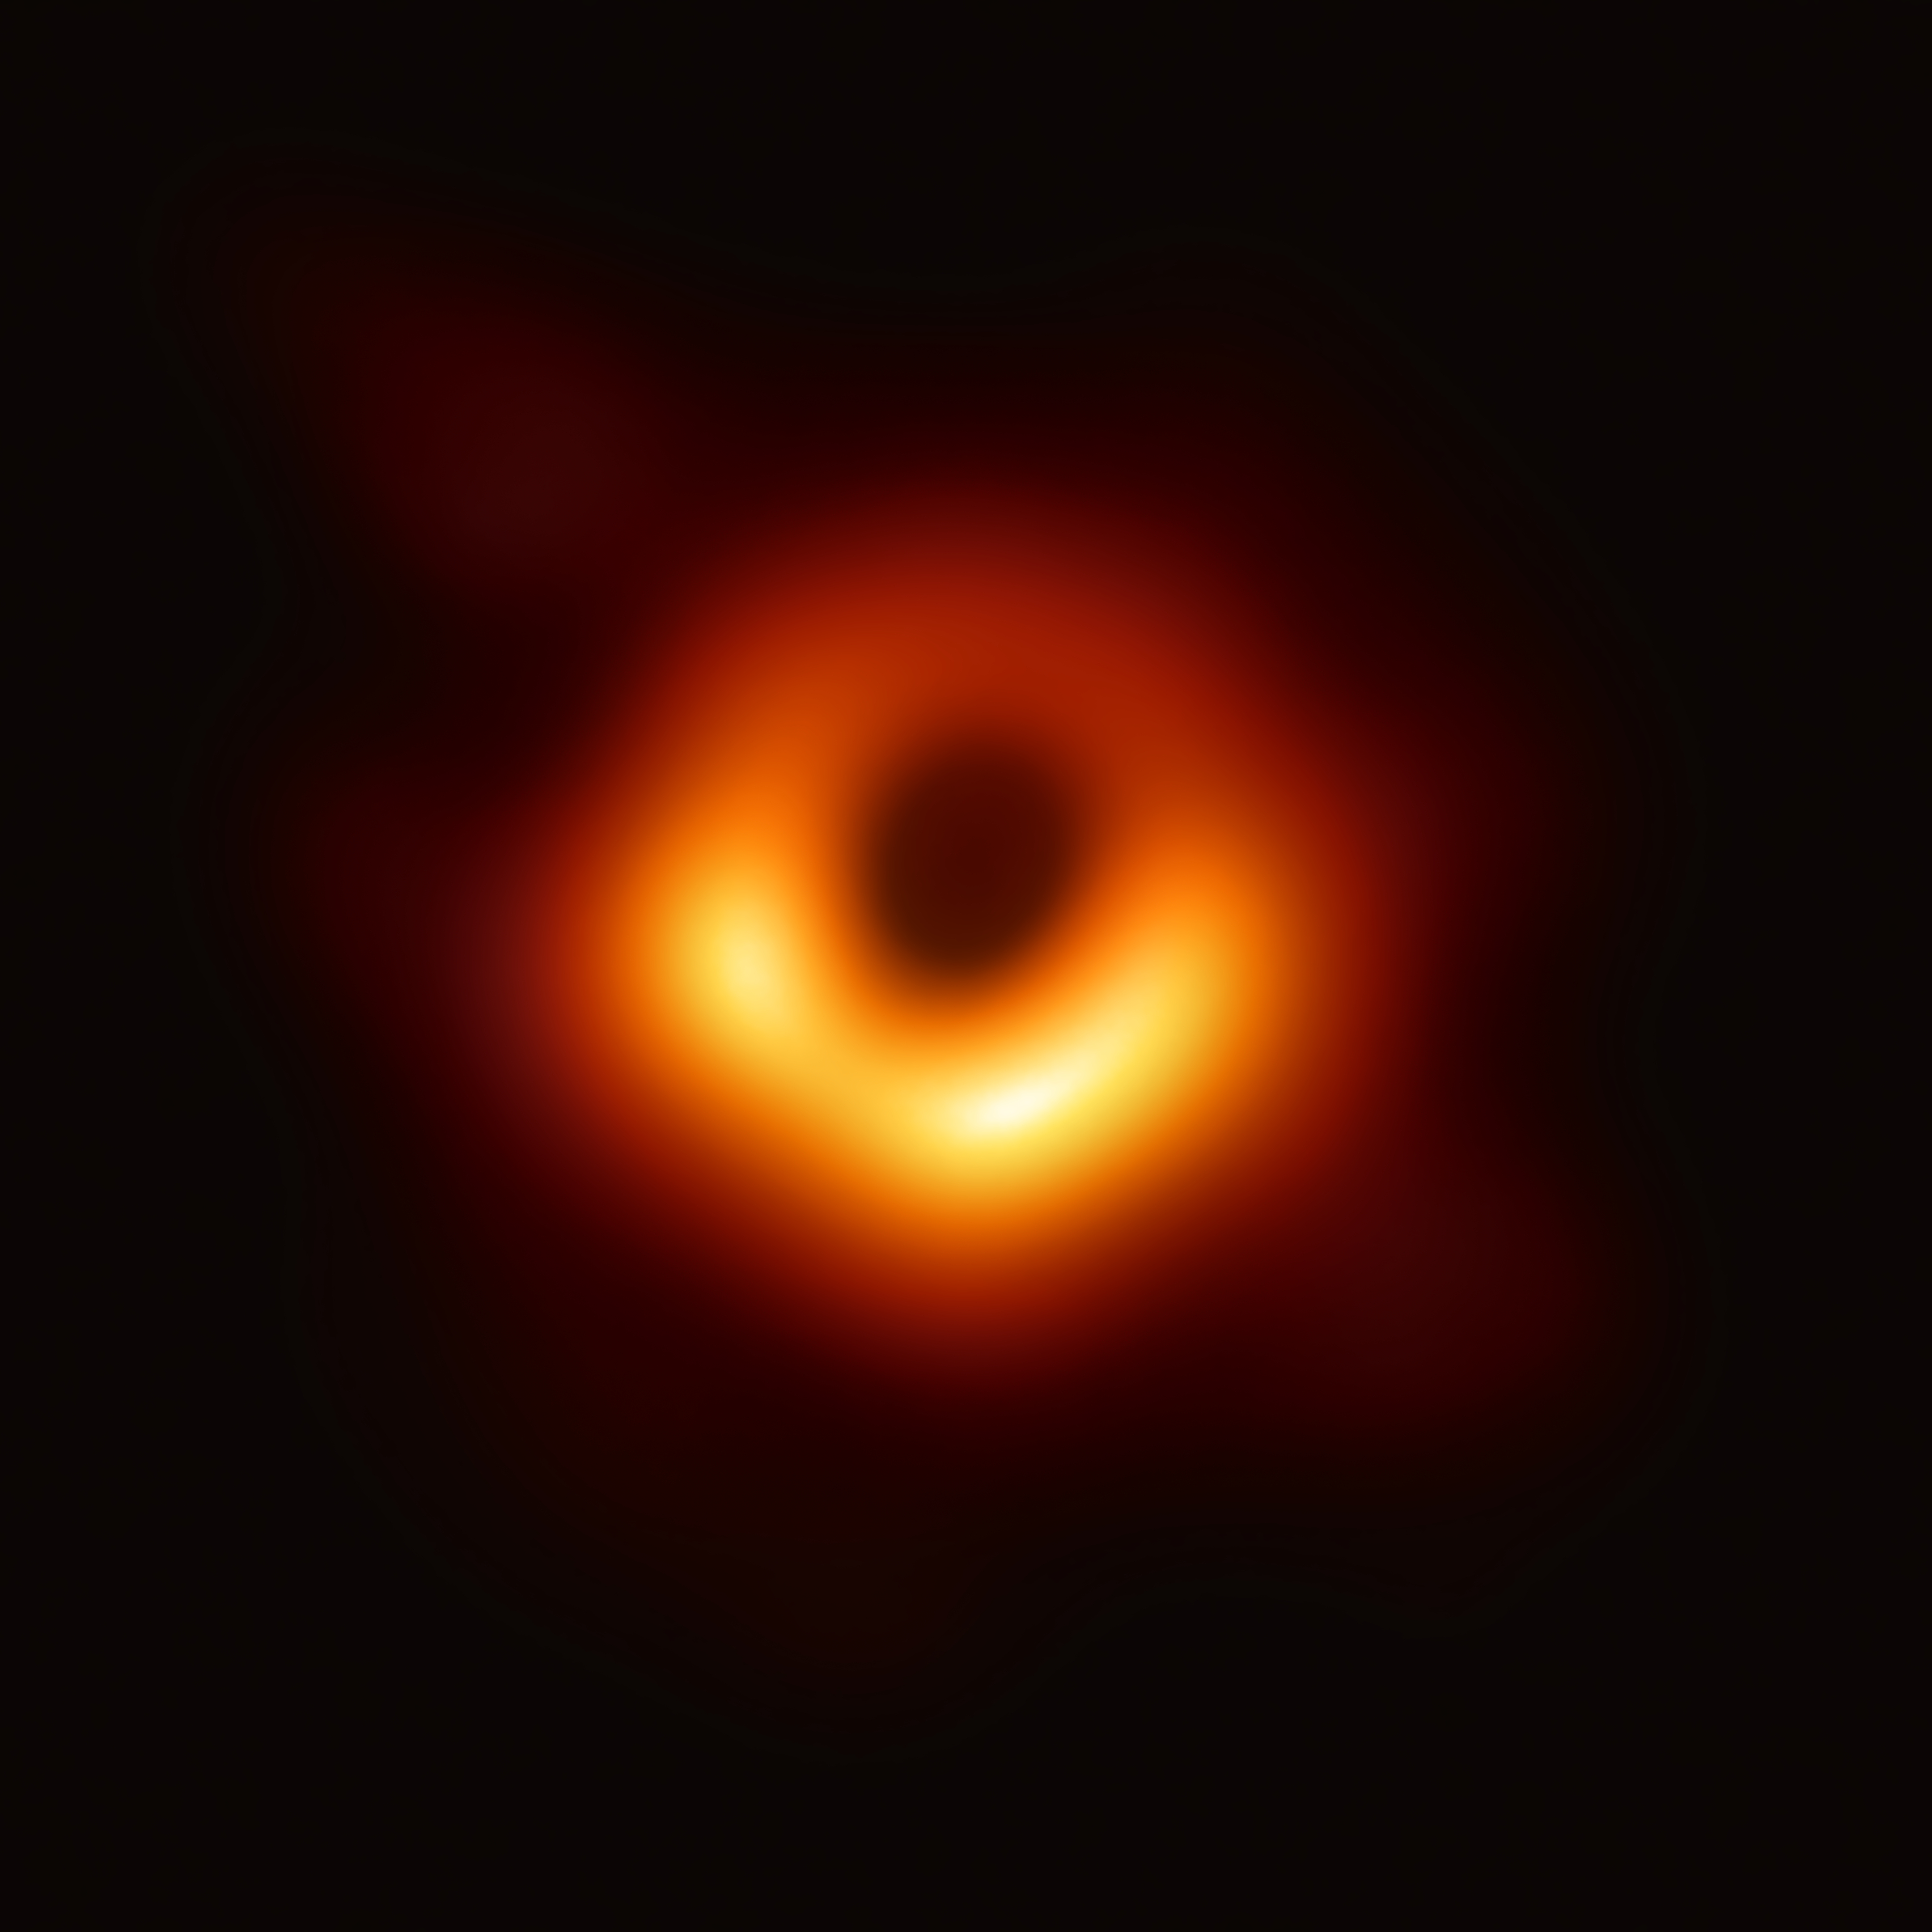
\includegraphics[width=5.0cm]{figs/Black_hole_-_Messier_87_crop_max_res.jpg}
        }
        \subfigure[银河系中心黑洞照片]{
            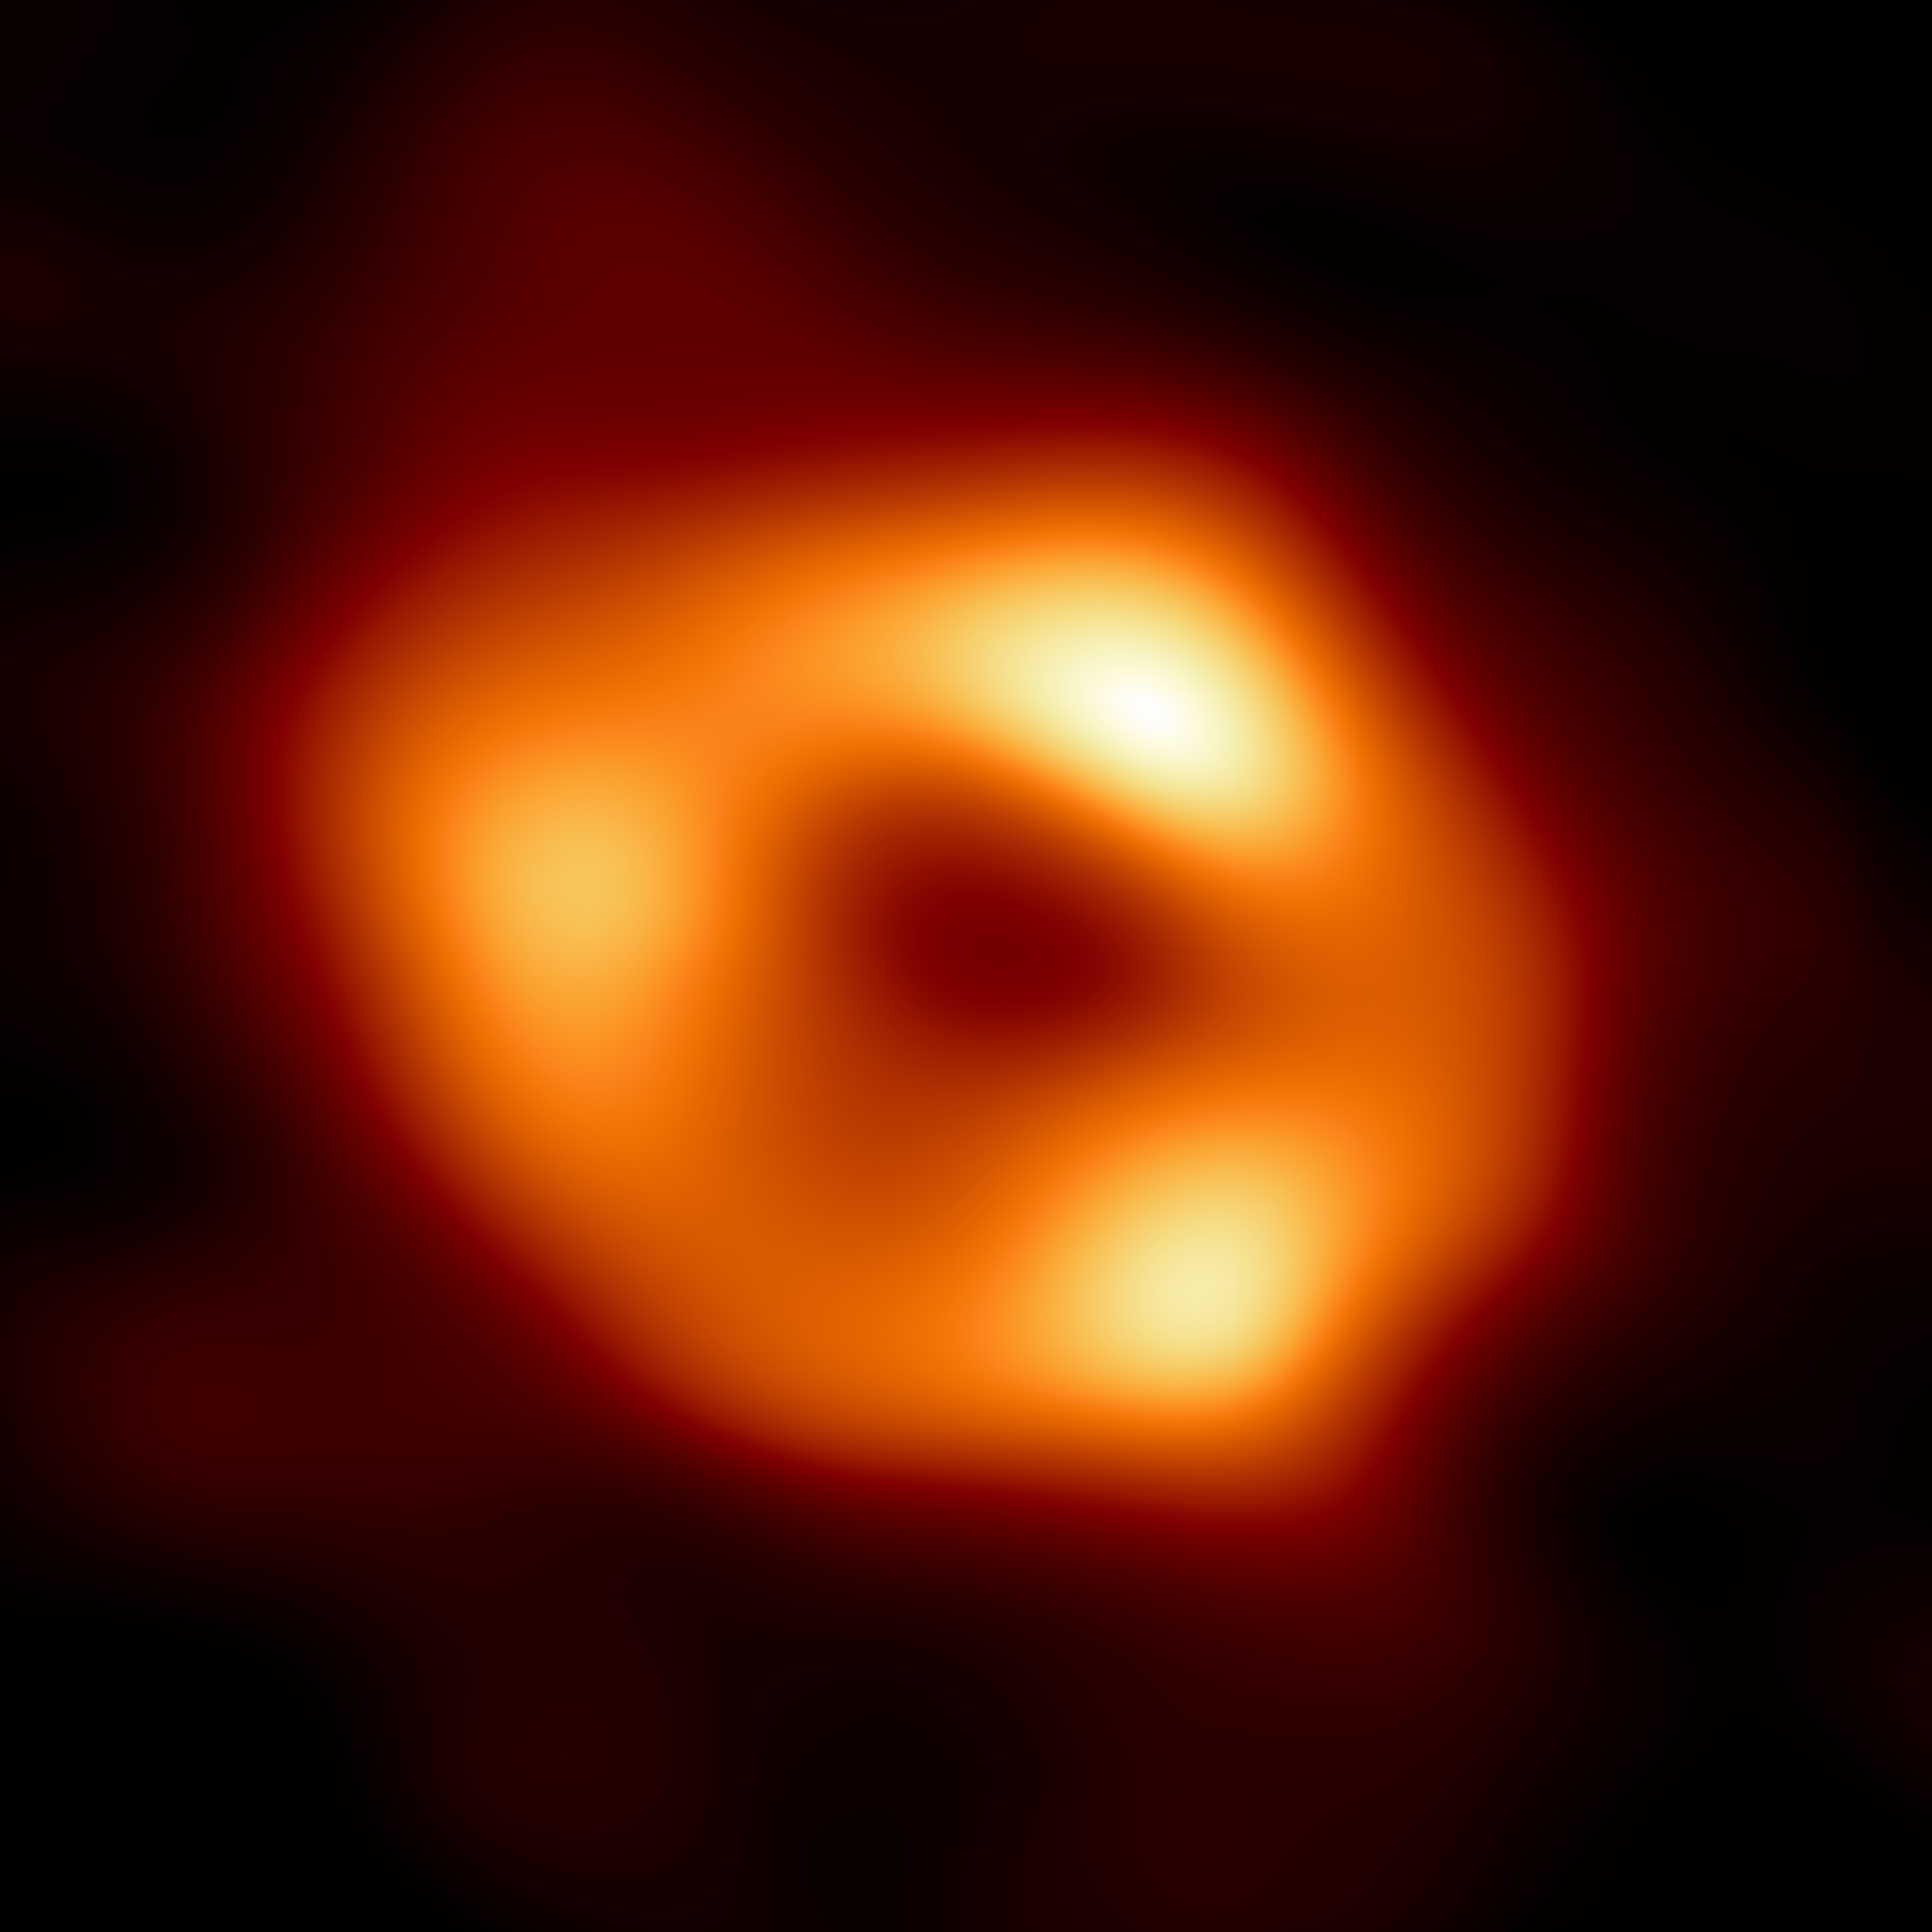
\includegraphics[width=5.0cm]{figs/EHT_Saggitarius_A_black_hole_converted_to_png.png}
        }
        \caption{黑洞照片}
        \label{fig:1}
    \end{figure}

    \subsection{关于黑洞名字由来的有趣轶事}
    1967年正值脉冲星被发现,在一场会议上,John Archibald Wheeler不停地使用了“引力塌缩星体”这个称呼,观众席下便有人提议简称为“黑洞”。后来在Wheeler的推崇下,1967年之后,
    学界正式将黑洞一词作为严肃的天体名称。\cite{siegfried201950}不过这个名字事实上也相当应景。“黑”表现了光无法逃逸,“洞”生动形象的指出了它的怪异,在时空这一弹性弯曲空间中就像是挖去了一个洞一样。
    冥冥之中,或许黑洞这一词也在致敬它的第一位研究者Schwarz,Schwarz是德国人,他的名字在德语中的意思正是“黑色的”!

    \section{掉入黑洞之前}
    现在假设我们乘坐飞船到了银河系中心,去近距离看看那里的黑洞。我们接近的是一个最简单的黑洞情形,不带电,也不旋转,因为旋转的黑洞会带来一些奇怪的效应,比如多个视界以及数学上的
    不稳定性,难以捉摸。不过你飞船上的伙伴可不想跟着你去送死,所以一直在飞船上看着你远去。
    \subsection{黑洞的吸积盘}
    我们首先似乎就遇到了一个棘手的问题,那就是我们可能会在被黑洞吞没之前被烧死!

    由于黑洞的强大引力,它便会俘获周围的星体和物质,形成一个绕其旋转的等离子体吸积盘。\cite{page1974disk}这个吸积盘转动的速度是非常之快的,甚至可以接近光速,所以吸积盘内的
    物质会相互摩擦产生湍流,导致吸积盘的温度升高。这样吸积盘便会不断向外辐射强大的能量,可见光、紫外光、X射线、$\gamma$射线等等各个波段都有。\cite{bl}这么大的照度会让我们瞬间失明,等离子体本身
    的温度也会达到数十亿度,所以或许在远处我们就失去了看见黑洞的能力,还未触碰到黑洞就已经被瞬间蒸发。
    
    现在假设我们穿了防护力极强的宇航服,可以免受黑洞吸积盘的干扰,我们再假设我们有一个遮光罩,能大大降低黑洞的亮度,让我们能看清细节。首先我们注意到黑洞的吸积盘是蓝色的,这或许和图\ref{fig:1}
    不一样,因为图\ref{fig:1}并不是按照真实看见的光的颜色着色的。人眼看见的是可见光,在可见光波段中,蓝紫色的能量最高,这正和吸积盘的特性相符合,另外,极高温的星球呈现蓝色、核反应堆中切伦科夫辐射的蓝色辉光
    也是这个道理。

    另外,黑洞看起来因该会一边比另一边更亮一些,\cite{fukue1988color}因为前面说了吸积盘相对于黑洞中心在高度旋转,根据光的多普勒效应:
    \begin{equation}
        \nu^\prime=\sqrt{\frac{c\mp v}{c\pm v}}\nu
    \end{equation}
    我们接受到的两边发来的光的频率是不一样的,向着我们运动的那一边的光的频率要更大一些,更加蓝,视觉上更亮。

    \subsection{引力透镜效应与吸积盘}
    你或许已经开始想象黑洞周围的吸积盘就如土星光环一样了,但这并不完全正确。事实上由于黑洞的引力透镜效应,黑洞吸积盘的背面会稍稍“翘起来”。\cite{fukue1988color}

    光在时空中沿着时空测地线前进,欧几里得时空中测地线是直线,所以我们日常生活中常常说“光沿直线传播”。但是广义相对论否定了这一观点,认为时空的本质是弯曲的,特别是黑洞
    这种极端天体,它附近的时空会被极度的弯曲,这个时候测地线就不是直线了。宏观上看光走的便是弯曲的路径(如图\ref{fig:2}),就像是经过透镜的光线被折射一样,这一现象最早在1919年被Eddington观察到,
    作为广义相对论的有力论据之一。
    \begin{figure}[H]
        \centering
        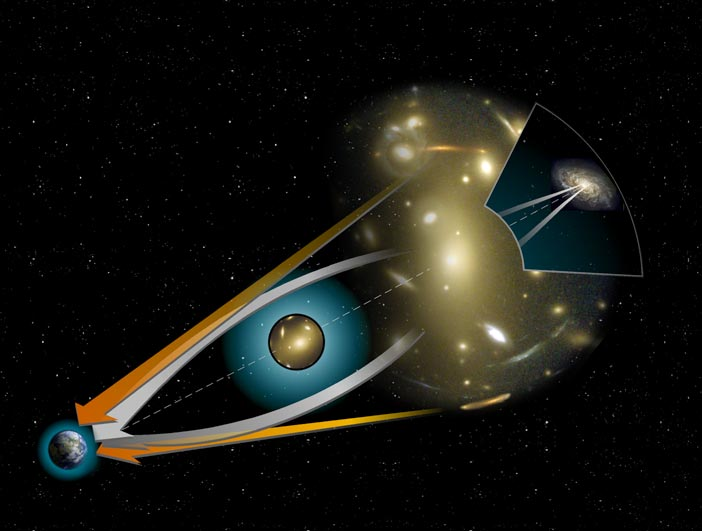
\includegraphics[width=7cm]{figs/Gravitational_lens-full.jpg}
        \caption{引力透镜效应图示}
        \label{fig:2}
    \end{figure}

    利用引力透镜效应,天文学家得以观察到许多大质量星体背后射来的光线,还可以发现奇特的星体的多重像现象。在这里黑洞的引力透镜效应是如此之强,导致其背后的吸积盘的光线在经过黑洞顶部时
    发生弯曲进入人眼,所以便产生了如电影《星际穿越》中的“卡冈图雅黑洞”的艺术概念图。(见下图\ref{fig:3})
    \begin{figure}[H]
        \centering
        \subfigure[星际穿越里面的卡冈图雅黑洞]{
            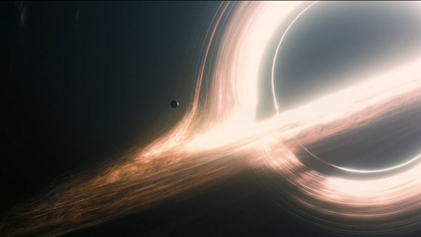
\includegraphics[width=5cm]{figs/Black_hole_Interstellar.png}
        }
        \subfigure[根据理论计算通过计算机渲染得到的黑洞真实图像\cite{Muller_2012}]{
            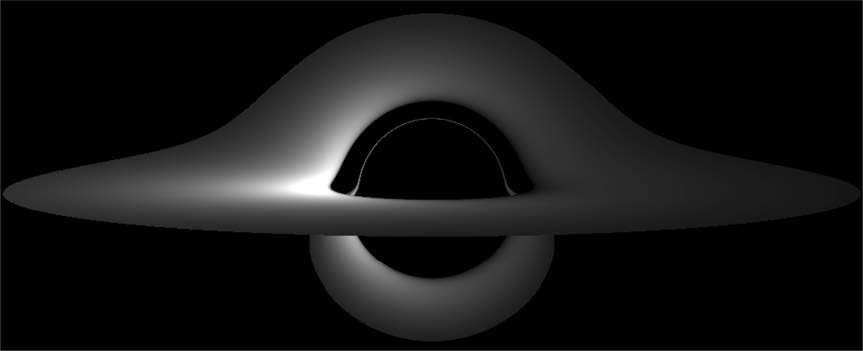
\includegraphics[width=5cm]{figs/black_hole.jpg}
        }
        \caption{黑洞的理论想象图片,这两幅图都没有还原真实人眼所见蓝色}
        \label{fig:3}
    \end{figure}
    \subsection{引力红移}
    另外,在黑洞附近你若是向外看,外面的星空中的恒星会变得“蓝”一些,这并非和哈勃红移一是由于恒星离我们远去导致的多普勒效应,而是黑洞扭曲时空进而扭曲了时间,
    是的我们的时间流逝的要比远处的恒星更加慢。那么,相对于我们而言,远处来的光线“看上去”像是加速了一样(当然光速本身是不变的),实际上会看到相反的“引力蓝移”现象,
    看到的外部恒星光线会更加偏蓝。\cite{florides2002einstein}
    
    值得一提的是,当初Einstein在1907年就早早地提出了这个效应,甚至早于广义相对论。\cite{valente2018einstein}因为在当初其实只需要使用等效原理就可以很好的解释了这一现象,
    而且在地球表面均匀重力场中,实际上也可以观测到这一现象。\cite{pound1959gravitational}
    \section{穿越吸积盘}
    \subsection{震惊!看起来竟然还越来越远?}
    接下来发生的事或许让你大吃一惊,因为你在刚刚开始坠落时,你看起来视野中的黑洞好像离你越来越远!但是放心,你确实在坠落,这一切的一切都是你的眼睛在欺骗你,
    你相对于黑洞在运动,所以黑洞附近的光线相对于你会被挤向前方,借用一个光学术语——像差。\cite{chang2020black}像差在天文观测中非常常见,人们总是想尽一切办法抵消它。你看起来正在远离黑洞正是由于像差,
    不过好在后面你下降的越来越快,一切又会恢复正常。
    \subsection{无聊下坠ing}
    有了特制宇航服的保护,剩下的就是无聊的下坠了。不过你若是想念飞船上的伙伴,还可以趁机多看几眼,不过你看到的景象会越来越暗淡,因为随着你下降的速度越来越快,你身后的光线会越难追上你,导致外面的星空
    看起来越来越黯淡。但是只要你还能看见飞船,现在回头还来得及,越过事件视界之后就后悔莫及了。因为,他会吞噬一切$\ldots$
    \section{飞跃事件视界}
    \subsection{何为事件视界?}
    一句话解释:事件视界在天体物理学中意味着事件不能影响观察者的边界。听起来似乎是比较抽象,其实对于施瓦西黑洞就是前面提到的施瓦西半径内,因为这一半径内连光线都无法逃脱,自然
    里面发生的任何事情都不会影响到飞船上的观察者。不妨看看这一过程中你飞船上的伙伴是什么反应。
    \subsection{飞船上的人眼中的你}
    对于你来说,跳进黑洞这一过程是一气呵成的下坠,不过对于你飞船上的伙伴,他们会看见你越来越慢的靠近黑洞,直到在某个位置定格不动,这个位置便是黑洞的事件视界,你之后落入事件视界所发生的一切事情
    都不会被你的伙伴知晓。你在接近黑洞的过程中,你发射出的光逃逸黑洞所需要的时间也在变长,你的伙伴这时看到的你是引力红移后的像,最后会在事件视界处慢慢的黯淡消失在整个宇宙中。你的伙伴可以离去了,
    因为在你此时越过事件视界后,他们再也不可能援救你。
    \subsection{光子球}
    我们回过头来再来看一下在即将抵达事件视界之前你会看到什么奇异的镜像。

    就像是环绕地球的卫星一样,在黑洞的事件视界附近存在一个区域,光子不至于落入事件视界中,但会被束缚在一个球面上环绕黑洞运动。在这个球形区域便是光子球,对于你即将着陆的施瓦西
    黑洞来说,这一半径为:
    \begin{equation}
        r=\frac{3GM}{c^2}=\frac{3}{2}r_s
    \end{equation}

    理论上这个时候你就像在照一个极端的哈哈镜一样,从你后脑勺发出的光线会绕黑洞运动一周然后进入你的眼睛。所以这个时候理论上你如果朝着你身体的一侧看,你应该就可以看到你的
    后脑勺。这一画面实在是过于诡异。

    光子球还有一个比较有意思的现象是感受到的离心力反转。\cite{abramowicz1990centrifugal}在光子球之外,一切正常,当你绕着黑洞旋转时,在你的旋转非惯性系下所感受到的离心力会
    随着你旋转速度的加快而变快,也就是常说的旋转的越快感觉自己身体向外甩的趋势越大。可在光子球上,这一趋势变为0,在光子球内部,这一趋势相反,你所感受到的是向心力而非离心力。
    \subsection{穿过光子球后大约$\SI[]{24}{s}$}
    费了九牛二虎之力,你终于安全的跨过了事件视界,不过这一安全显然是暂时的。

    实际上穿越事件视界后你啥也感觉不到,或者说你根本无法判断你是否已经抵达事件视界,因为虽然外面的光线会全部被吸入黑洞无法逃脱,但是相对于正在下落的你而言还是能进入你的眼睛,
    所以你还是能看见远处的恒星,看见飞船上的伙伴们。其实上这也可以基于一个基本常识加以解释。虽然黑洞周围的时空弯曲的厉害,但是在任何一个局部,都还是近似于平坦的,就单纯你所在的那一小块,
    时空的曲率是完全可以忽略的,所以你不会感受到任何异常。而且根据计算,同样是因为像差,黑洞仅仅只会占你视野中的$15\%$,而且你会看到你的飞船会越来越大,就像是在靠近他们一样。当然,这一切又是你的眼睛和
    你耍的小把戏。

    我们这里考虑的是无自旋的施瓦西黑洞。万一黑洞在旋转,事件视界之外的空间实际上都会围绕黑洞运动,也即“参考系拖拽效应”。早在1918年人们就注意到了这一现象。\cite{thirring1918effect}
    值得庆新的是你不需要面对这一过程。
    \subsection{意大利面条}
    在我们即将到达黑洞中心时,我们自身的尺度下的时空曲率已经足够大到无法像刚才一样忽略了。就像是潮汐力一样,我们的头相对于脚离黑洞更远,由于黑洞周围时空极度的弯曲,
    在你的身高尺度下,头和脚所受到的引力有很大的不同,从而引力会把你越拉越长,就像是意大利面条一样。\cite{time}所以理论上来说,较矮的人相对来说撑的更久一些。。。

    \section{黑洞中心}
    你本人自然是无法达到黑洞中心了,不过幸运的是你的身体碎片可以代劳。
    \subsection{令人担忧的时空奇点}
    现有的理论预言了黑洞导致的时空奇点的存在。这个奇点的存在是非常令人困惑的,因为所有的物理定律在奇点附近全部失效,我们无法预言在离黑洞中心如此之进的范围内将会发生什么。
    之前曾提到过Einstein认为大统一理论能完全解释时空奇点。这一观点现在也卷土重来,相信人类终有一天会实现统一理论的构建!
    \subsection{黑洞的未来}
    Hawking在1974年预言黑洞会向外缓慢的辐射能量,最终完全蒸发为光子。当然这一过程是非常缓慢的。Hawking证明这一观点时所用的工具是弯曲时空中的量子场论,不过他在他自己的著作《时间简史》
    中给了一个比较形象的说明\cite{time}:

    {\itshape“一对在黑洞事件视界附近产生的正反虚粒子,一个不小心掉进了黑洞,而另一个却成功逃逸,变成了一个实粒子。”}

    这一论述优雅简洁,令我印象深刻。可惜真实的理论比这要复杂的多。Hawking也主要是为了照顾其科普书的主要受众知识水平而将原始理论变成了这副模样。但不可否认它确实
    让人们直观的感受到了霍金辐射的存在性。

    那么转念一想,最终你的身体碎片会随着黑洞的慢慢蒸发从而回归宇宙。这难道不是免费的一场高级宇宙葬吗?!
    \subsection{我们所不知道的事}
    关于黑洞的一切我们实在是知道的太少。比如霍金所建立的黑洞热力学第二定律提出的黑洞熵仅仅与事件视界面积成比例:
    \begin{equation}
        S=\frac{1}{4}\frac{c^3k_B}{G\hbar}A
    \end{equation}
    和大家预想到的应该与体系体积成比例不一样,这也促使Gerard't Hooft 和 Leonard Susskind提出了引力全息理论。\cite{hooft2001holographic}关于黑洞的研究和弦理论也走的越来越近,人们愈发希望
    通过统一广义相对论和量子场论(量子引力论)从而解释这些奇异的现象。

    再比如火热的黑洞信息悖论,不断有新的奇特的理论提出来解决这些问题,比如黑洞互补理论。也有新的悖论提出来否定解释黑洞信息悖论的理论,比如2012年的\textbf{火墙悖论(firewell paradox)}。\cite{almheiri2013black}
    这个理论恰巧就是考虑我们所考虑的情形,广义相对论显然认为我们会一直坠入奇点最终被扯成碎片。不过火墙悖论认为,由于量子效应,黑洞的事件视界会变成一个极高能区域,就像一面“火墙”一样,任何东西一触即焦,这也是这个悖论的名称由来。
    这个理论质疑了我们能否顺利越过事件视界。

    \section{尾声}
    我们从最初的黑洞理论的雏形开始,大致上预测了你若不幸掉入黑洞会发生什么。不过这里面的内容很多都还是有争议的,等待着新的理论来改进。比如狭义相对论提出后,人们想当然的认为以接近光速
    运动的你看到的世界应当由于尺缩而变小。但实际上直到狭义相对论发表大致五十年后,人们才意识到由于光线传播需要时间,以及尺缩的本质,才正式提出真实看到的景象应该是绕天球的旋转\cite{terrell1959invisibility},当然还要顺带考虑多普勒效应。
    
    所以人类对于宇宙探索的脚步从未停止,期待着未来会出现全新的黑洞理论推翻本文的绝大部分内容,这也证明了人类的不断进步!
    
    总之,目前来看,人类对黑洞下定论还为时太早,我们还有很长的一段长征路需要走。

    \nocite{*}
    \bibliographystyle{plain}
    \bibliography{ref}
\end{document}